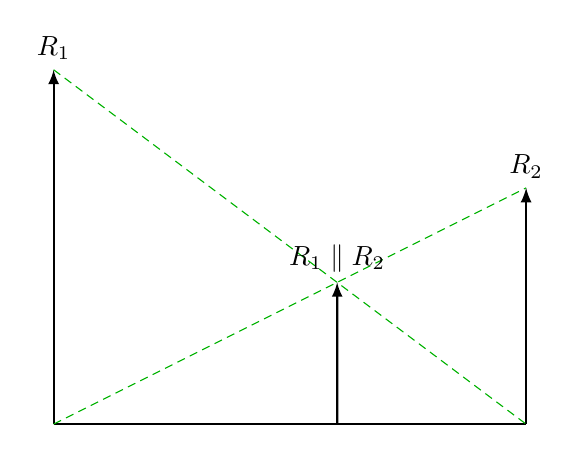
\begin{tikzpicture}[scale=1.5]
\coordinate (0) at (0,0);

\draw[thick, -latex] 	(0) -- ++(0,3) coordinate (1);
\draw[thick] 		(0) -- ++(4,0) coordinate (2);
\draw[thick, -latex] 	(2) -- ++(0,2) coordinate (3);

\draw[densely dashed, green!70!black]
	(1) -- (2)
	(0) -- (3);
				
\node[above] (A) at (1) {$R_1$};
\node[above] (B) at (3) {$R_2$};
\node[above] (C) at (intersection of 1--2 and 0--3) {$R_1 \parallel R_2$};

\draw[thick, -latex] (0 -| C) -- (C);
\end{tikzpicture}